\documentclass[11pt,a4paper]{article}
\usepackage[margin=2.3cm]{geometry}
\usepackage{booktabs}
\usepackage{graphicx}
\usepackage{amsmath}
\usepackage{xcolor}
\usepackage{tcolorbox}
\usepackage[colorlinks=true,linkcolor=blue,urlcolor=blue]{hyperref}

\title{Simulating a hanging cable:\\
       mathematics, measurement, and three solvers compared}
\author{Generated by \texttt{analysis/make\_thesis\_report.py}}
\date{\today}

\begin{document}
\maketitle

\begin{abstract}
A flexible cable is suspended from 3 level clamps spanning
$S = 0.350$\,m and photographed. Its shape is predicted three independent
ways: from the governing differential equation, from a set of physics solvers,
and from the photograph itself. The three-way structure is deliberate --- any
two of them can agree for uninteresting reasons, and only the third makes it
possible to attribute a disagreement to numerical error rather than to
modelling error. This document reports what agrees, what does not, and which
results are currently trustworthy.
\end{abstract}

\section*{Summary of findings}
\begin{itemize}
  \item The governing equation, integrated numerically without recourse to its closed form, reproduces $z = a\cosh((x-x_0)/a)+c$ to $7\times10^{-3}$\,\textmu m. The analytic reference every error here is measured against is therefore verified rather than assumed.
  \item Newton cable - point pin (kink) reproduces the analytic catenary to 0.91~mm on a 893~mm cable (0.26\% of the span).
  \item Agreement with the mathematics and agreement with the photograph rank the solvers in opposite orders. The gap measures the difference between a clamped and a pinned end, not solver accuracy.
  \item Imposing the real (flat-tape) middle boundary condition rounds the kink and moves the Newton cable from 75~mm to 65~mm against the photograph, while raising its error against the idealised catenary from 0.9~mm to 21~mm --- confirming the residual is a boundary condition, not solver error.
  \item Solver accuracy depends on the PRODUCT of substeps and iterations, but cost does not: each substep carries fixed overhead an iteration does not, so fewer substeps with more iterations is strictly cheaper at equal accuracy.
  \item Damping the stretch constraint is actively harmful --- it opposes the solver's own length correction --- while damping the bending constraint does nothing measurable across a $600\times$ range.
  \item The Warp rod is the only method imposing a true position-only pin, so its shape depends on the one input this study cannot measure: the bending stiffness. Its error against the catenary rises from $53$~mm at the cable's drape-consistent $\ell\approx20$~mm (used here) to $80$~mm at the stand-in material's $\ell\approx150$~mm. At coarse resolution the stiff case additionally buckles into an arch $150$~mm above the supports; refining the mesh removes the buckle, so that was a discretisation artefact while the stiffness sensitivity is not.
\end{itemize}

\section{Apparatus}

The cable is clamped with tape to a vertical door at
0.000 m, 0.150 m, 0.350 m
measured from the leftmost clamp, all at one height, and photographed
square-on. Cable length is not taken from the packaging: the free length
between clamps is what governs the shape, so it is measured from the same
photograph the simulations are compared against. Here that gives
$L = 0.8932$\,m, and $L/S = 2.552$ --- a very slack
cable, sagging further than it spans.


\begin{figure}[htbp]
  \centering
  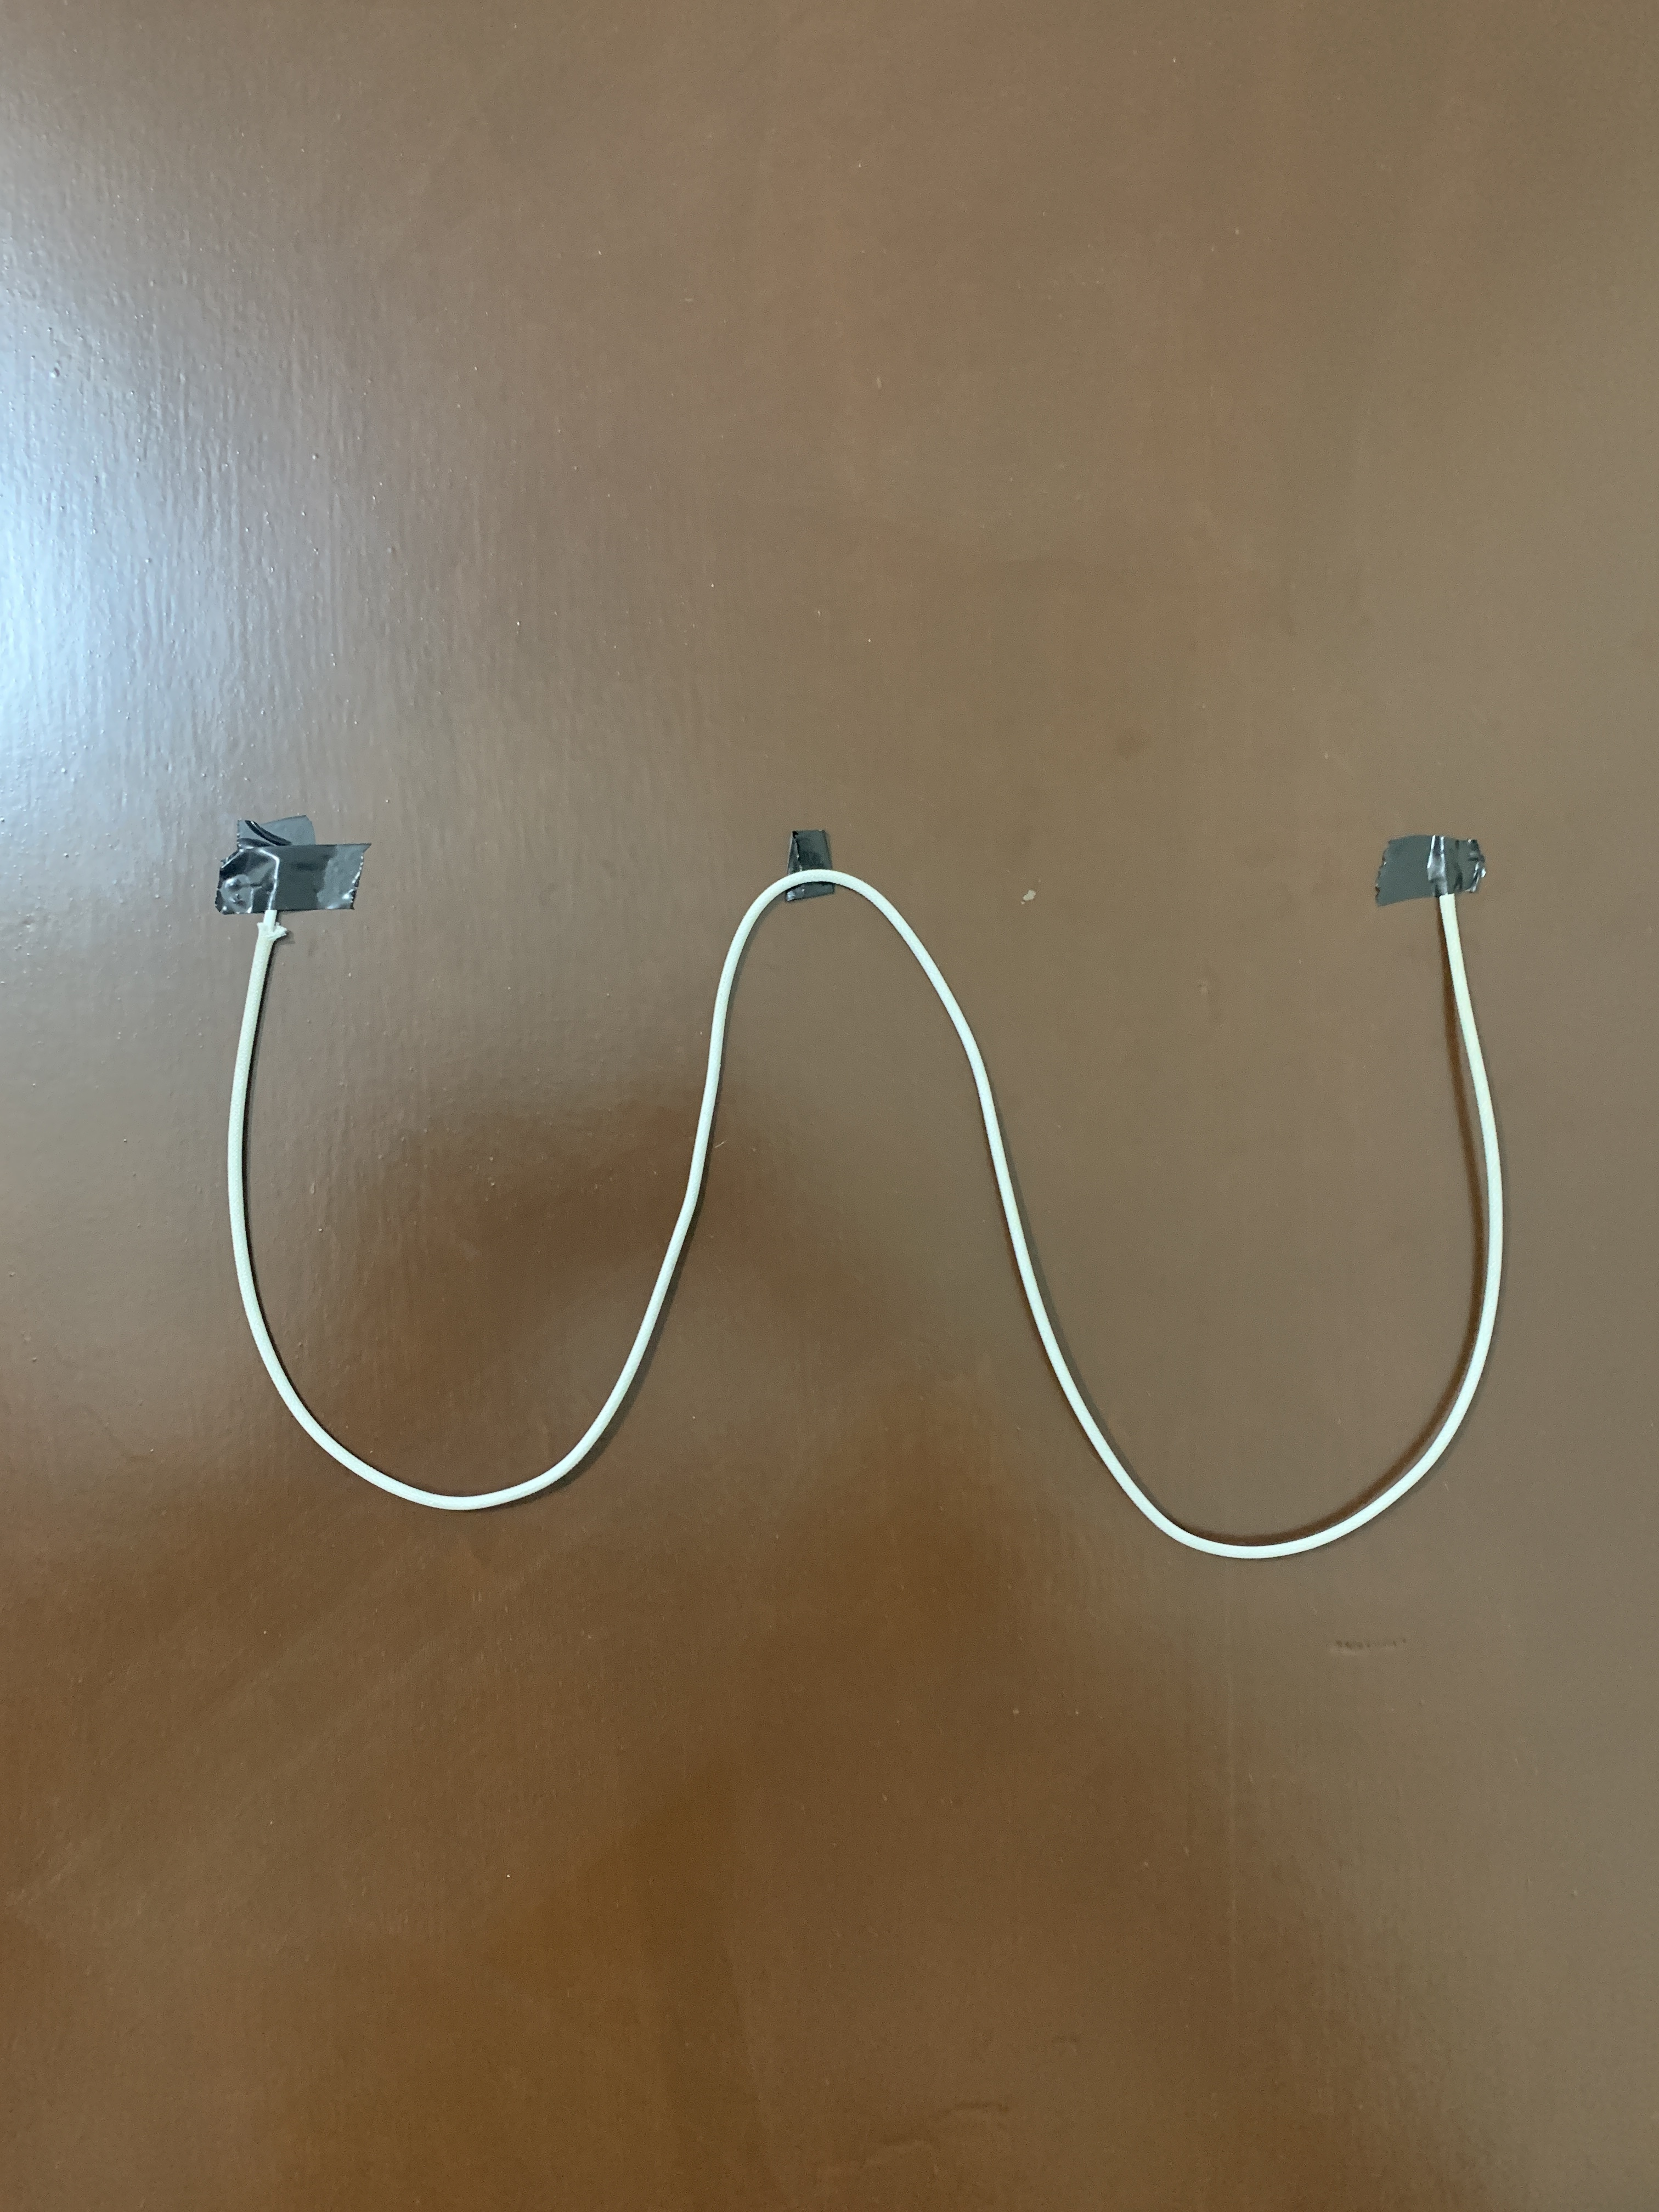
\includegraphics[width=0.62\linewidth]{photo.jpg}
  \caption{The cable as photographed. The tape fixes the cable's ANGLE as well as its position, which is a clamped boundary condition, not the pinned one the classical catenary assumes.}
  \label{fig:photo}
\end{figure}


\section{Image processing}

The cable is separated from the door in HSV: it is bright and nearly
unsaturated where the door is a saturated brown. The connected component is
then selected by SHAPE rather than by area --- a specular highlight on the door
is also bright and unsaturated, and is often \emph{larger} than the cable, so
selecting the largest region finds the glare instead. A cable is thin and spans
the clamps; glare is a blob.

The centreline is then traced ALONG the curve: from each point the tracer
advances one step along the local tangent and re-centres on the mask's
perpendicular cross-section. The obvious alternative --- averaging the mask
rows in each pixel column --- fails badly here, because a slack cable hangs
near-vertically close to its clamps and one column then spans a long run of
cable. Figure~\ref{fig:detection} is the check on all of this: the left panel
tints every segmented pixel so a mis-segmentation is visible directly, and the
right panel compares the extracted profile to a fitted catenary, because a
clean segmentation can still fit badly and those are different failures.


\begin{figure}[htbp]
  \centering
  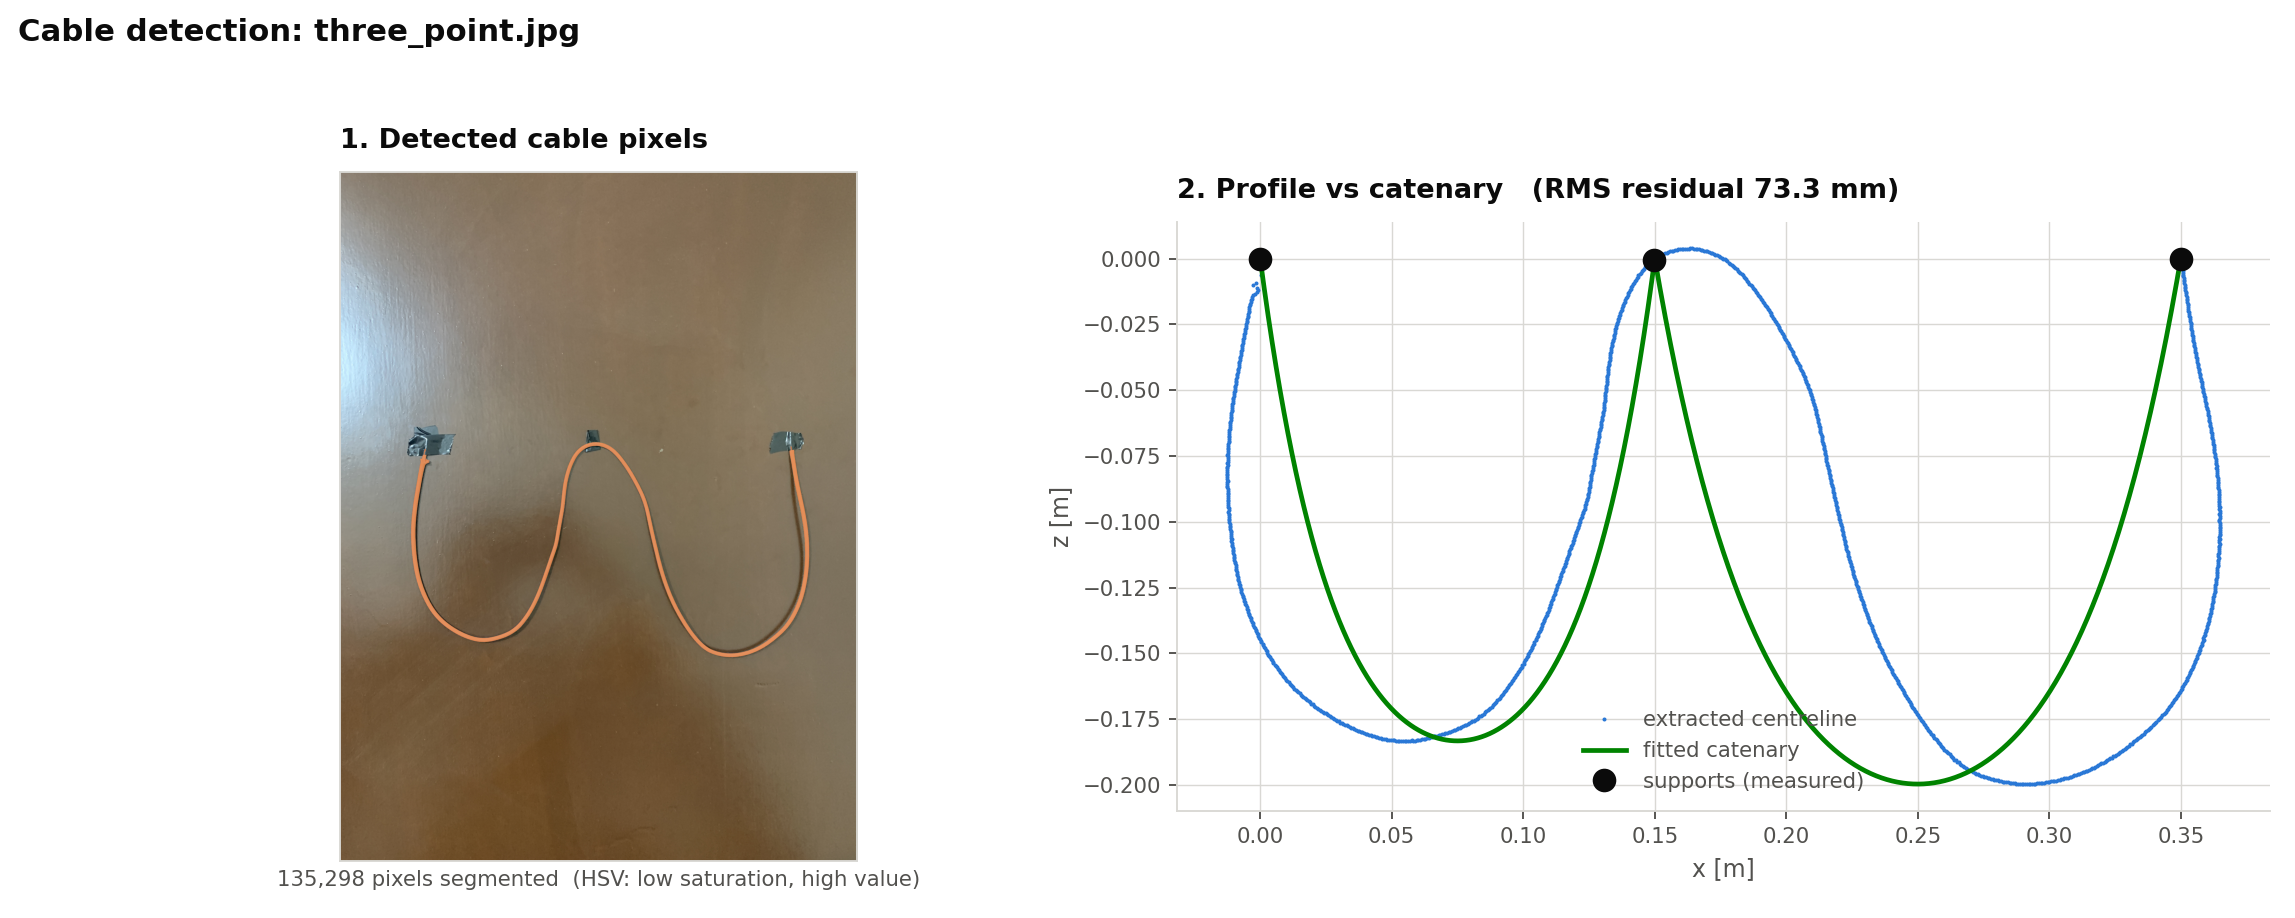
\includegraphics[width=\linewidth]{detection.png}
  \caption{Detection and fit. Left: every segmented pixel, tinted over the original. Right: extracted profile against the fitted catenary.}
  \label{fig:detection}
\end{figure}


\section{Mathematical model}

For a perfectly flexible, inextensible cable of weight $w$ per unit length, the
horizontal component of tension is constant along the cable, $T\cos\theta = H$.
Balancing the vertical forces on an element $\mathrm{d}s$ and substituting
$\mathrm{d}s = \sqrt{1 + z'^2}\,\mathrm{d}x$ gives the governing equation
\begin{equation}
  z'' = \frac{\sqrt{1 + z'^2}}{a}, \qquad a = \frac{H}{w},
  \label{eq:catenary}
\end{equation}
a two-point boundary-value problem closed by the arc-length constraint
$\int_0^S \sqrt{1 + z'^2}\,\mathrm{d}x = L$, which is what fixes $a$.
Physically $a$ is set by how much cable was hung: a slacker cable has a smaller
$a$ and therefore carries \emph{less} tension.

The corresponding dynamics, which is what the solvers actually integrate, is
\begin{equation}
  \rho A \frac{\partial^2 \mathbf{r}}{\partial t^2}
    = \frac{\partial}{\partial s}\!\left( T \frac{\partial \mathbf{r}}{\partial s} \right)
      + \rho A \mathbf{g},
  \label{eq:dynamics}
\end{equation}
with $|\partial \mathbf{r} / \partial s| = 1$ enforced by $T$, which is a
Lagrange multiplier rather than a material property. Setting
$\partial^2\mathbf{r}/\partial t^2 = 0$ recovers~\eqref{eq:catenary}, which
is the assumption that licenses scoring a settled simulation against the static
solution.

\paragraph{Verification.} Equation~\eqref{eq:catenary} is integrated
numerically (RK4 from the vertex, bisection on $a$ for the length constraint)
without using the closed form $z = a\cosh((x-x_0)/a) + c$ anywhere. The two
agree to $7\times10^{-3}$\,\textmu m. The analytic reference every error in
this document is measured against is therefore verified rather than assumed.

\section{Simulation}

Each solver runs in its own process --- Isaac Sim's \texttt{SimulationApp} is
a singleton and the methods force different physics engines --- and each is
handed the identical scenario file, so a method that disagrees is disagreeing
about physics rather than about its inputs.

\begin{table}[htbp]
\centering\small
\begin{tabular}{lrrrrcr}
\toprule
method & RMSE [mm] & max [mm] & sag [mm] & arc drift [\%] & settled & wall [s] \\
\midrule
    Newton cable - point pin (kink) & 0.91 & 2.94 & 220.7 & 0.855 & yes & 12.9 \\
    Newton cable - tape (rounded) & 21.12 & 72.65 & 218.3 & 1.064 & yes & 11.7 \\
    PhysX capsule chain (D6) & 74.40 & 150.39 & 204.0 & 0.457 & NO & 29.0 \\
    Warp XPBD rod & 44.78 & 96.60 & 212.4 & 0.133 & yes & 1.3 \\
\bottomrule
\end{tabular}
\caption{Each solver against the analytic catenary. Arc drift is the
reference-free check: an inextensible cable must keep its length whatever the
catenary says.}
\end{table}

\paragraph{Boundary conditions are not a detail.} These runs do not all hold
the middle support the same way, and the choice moves the shape more than the
solver does. The Newton cable appears twice, as the same solver under two
boundary conditions: \emph{point pin} welds the cable at the catenary's own
angle, which corners into a kink; \emph{tape} holds a short flat plateau, so
the cable leaves horizontally and its bending rounds the top, as a real strip of
tape does. The PhysX and Warp methods pin the node and let the cable pivot. The
point pin is nearest the analytic curve and the tape nearest the photograph ---
the same trade-off the conclusions turn on (Section~\ref{sec:conclusions}) ---
so the table compares \emph{models}, not solver quality. The middle clamp was measured to hold 46.9\% of the cable's arc length on its left, where the chord-proportional convention assumes 42.9\% (+4.0~percentage points). Since the clamp pins a material point, this split is a property of the apparatus rather than something statics determines, so it must be measured and imposed.


\begin{figure}[htbp]
  \centering
  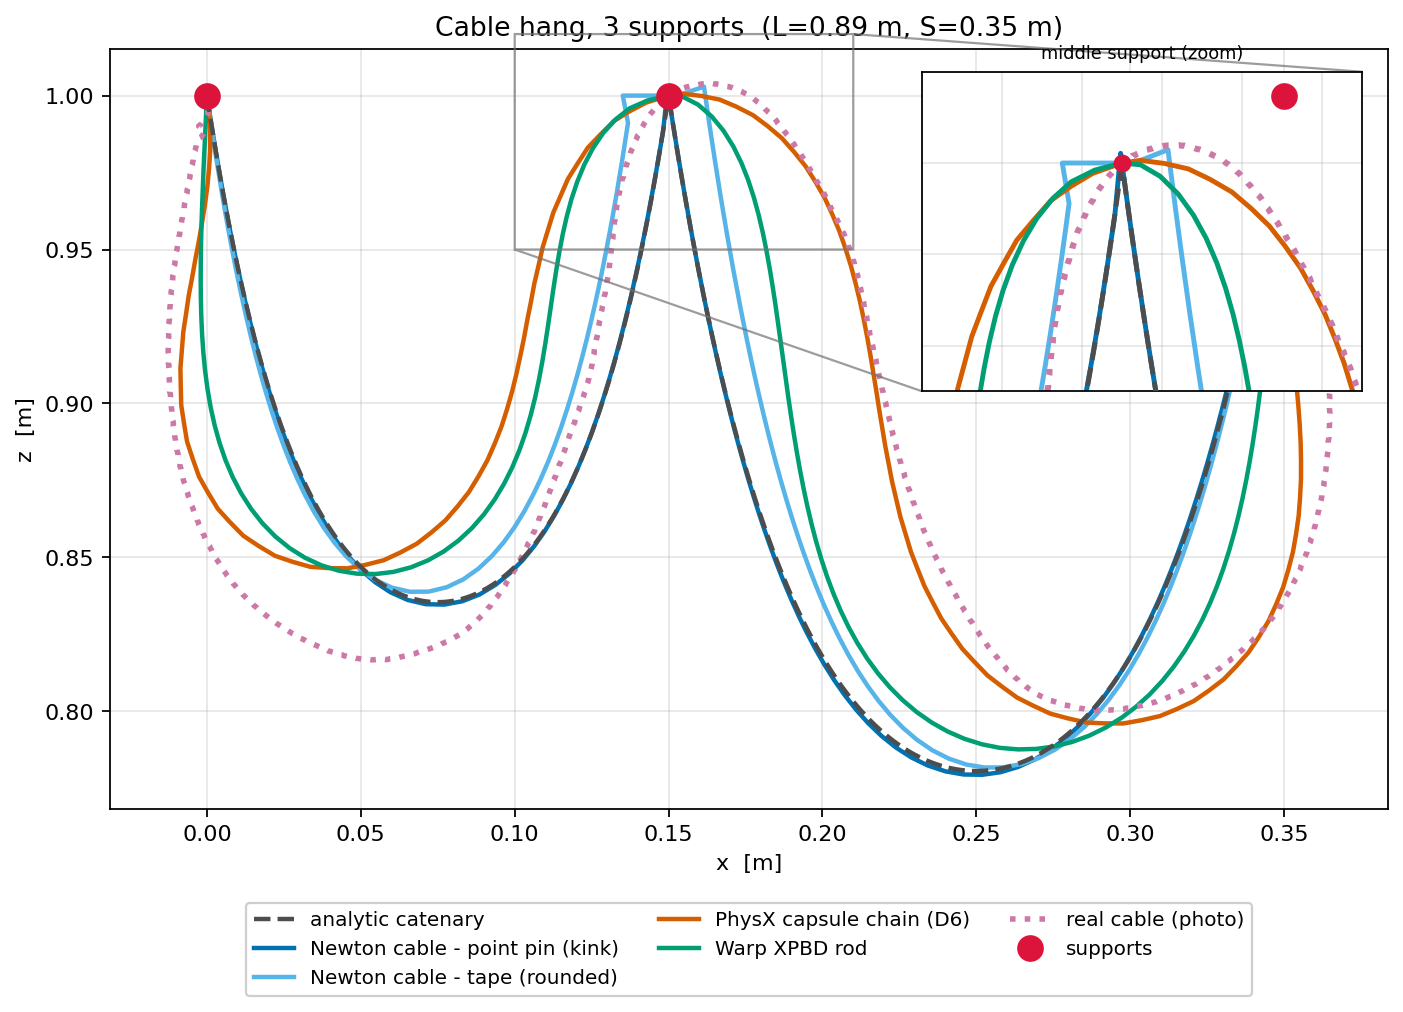
\includegraphics[width=\linewidth]{overlay.png}
  \caption{All methods, the analytic catenary, and the photographed cable on one axis. Inset: the middle support magnified. The point pin and the analytic catenary corner in an upward kink; the flat-tape model and the real cable both round over. That contrast is the boundary-condition result of Section~\ref{sec:conclusions} made visible.}
  \label{fig:overlay}
\end{figure}



\begin{figure}[htbp]
  \centering
  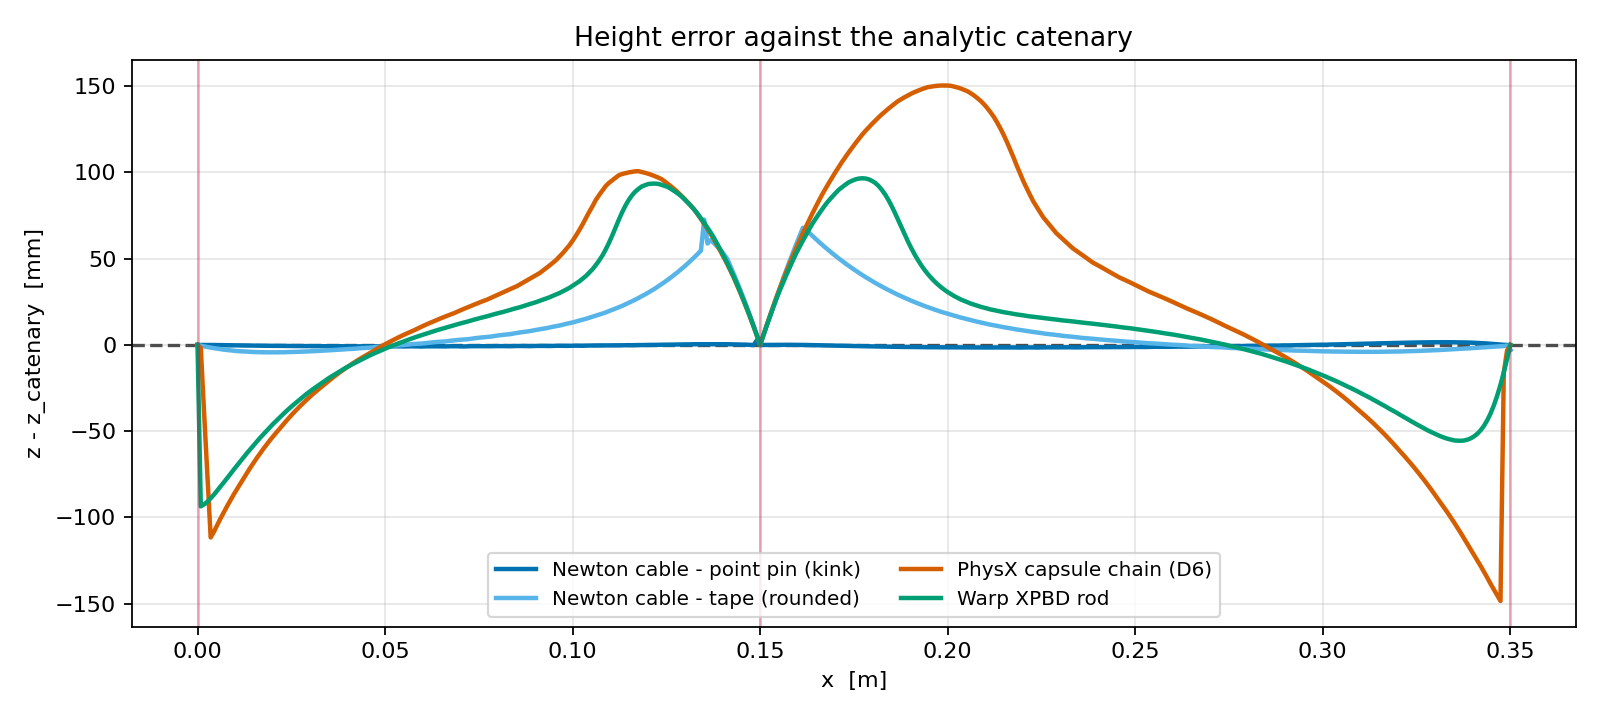
\includegraphics[width=\linewidth]{errors.png}
  \caption{Deviation from the analytic catenary along the cable.}
  \label{fig:errors}
\end{figure}


\begin{table}[htbp]
\centering\small
\begin{tabular}{lrr}
\toprule
method & RMSE vs photo [mm] & max [mm] \\
\midrule
    Newton cable - point pin (kink) & 75.10 & 159.59 \\
    Newton cable - tape (rounded) & 65.31 & 159.20 \\
    PhysX capsule chain (D6) & 32.77 & 156.36 \\
    Warp XPBD rod & 51.16 & 151.45 \\
\bottomrule
\end{tabular}
\caption{Simulation against the photographed cable. The extraction's frame is calibrated on the two outer clamps, which are level in the apparatus; the middle clamp is recovered to within 14~mm as an independent check (Section~\ref{sec:validity}), which bounds the accuracy of these figures.}
\end{table}

\section{Solver hyperparameters}

\paragraph{Robustness across slackness.} The sweep was run at two geometries
--- $L/S = 1.25$ and the photographed $L/S = 2.55$, twice as slack --- and
the conclusions are the same in both. Newton's default reaches $27.8$\,mm at
the lower slackness and $12.5$\,mm at the higher, both an order of magnitude
worse than a well-chosen budget; the $4\times200$ configuration is the best
accuracy-per-second in each; and the most accurate configuration lands at
$1.3$\,mm regardless. That the ranking survives a doubling of slackness is
evidence the guidance is about the solver rather than about one operating
point. The table below is the $L/S = 2.55$ case, matching the photograph.

Every cable example shipped with Newton uses $10$ substeps and $5$ iterations.
Applied to this problem that is far too coarse; but the repository's previous
default of $8 \times 200$ was tuned by varying iterations alone, leaving the
substep axis untested. A sweep over both, scored against the analytic curve,
shows accuracy to be essentially a function of the \emph{product} --- while
cost is not, because each substep carries fixed overhead that an iteration does
not. Fewer substeps with more iterations is therefore strictly cheaper at equal
accuracy.

Separately, damping the stretch constraint proved actively harmful: it opposes
the solver's own length correction, and raising it to $10^{-2}$ cost roughly a
factor of six in accuracy for no benefit. Damping the \emph{bending}
constraint, by contrast, changed nothing measurable over a $600\times$ range,
because this cable's $EI$ is small enough that the bending mode carries almost
no energy.

\begin{table}[htbp]
\centering\small
\begin{tabular}{rrrrrr}
\toprule
substeps & iterations & budget & RMSE [mm] & arc drift [\%] & wall [s] \\
\midrule
    4 & 5 & 20 & 36.79 & 12.09 & 6.8 \\
    10 & 5 & 50 & 12.50 & 4.14 & 11.4 \\
    4 & 200 & 800 & 1.51 & 0.43 & 26.2 \\
    8 & 200 & 1600 & 1.23 & 0.29 & 203.7 \\
    10 & 200 & 2000 & 1.31 & 0.27 & 267.3 \\
    16 & 200 & 3200 & 1.64 & 0.23 & 433.9 \\
\bottomrule
\end{tabular}
\caption{Selected configurations from the sweep.}
\end{table}


\begin{figure}[htbp]
  \centering
  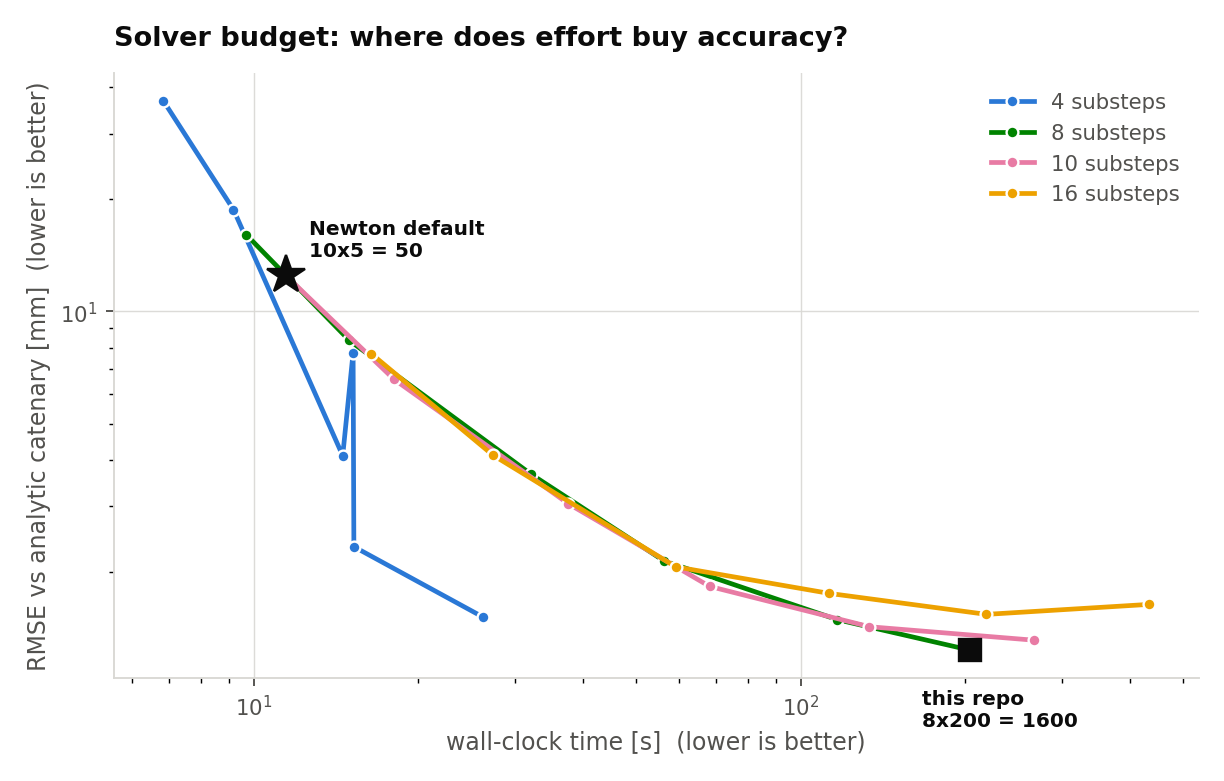
\includegraphics[width=\linewidth]{budget.png}
  \caption{Accuracy against wall-clock cost. Both axes logarithmic; the knee is where further cost stops buying accuracy.}
  \label{fig:budget}
\end{figure}



\begin{figure}[htbp]
  \centering
  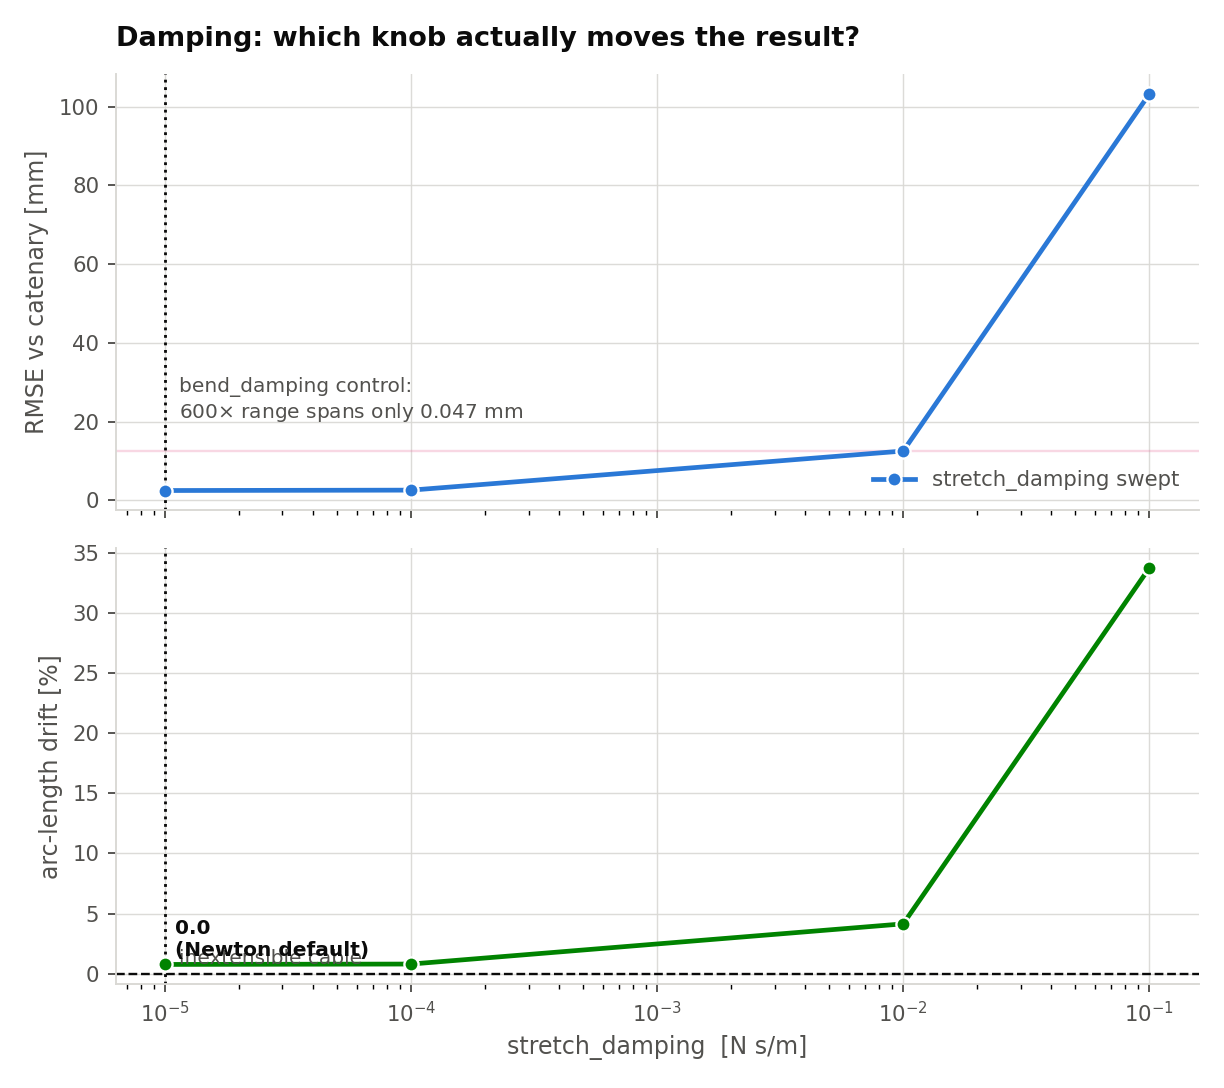
\includegraphics[width=\linewidth]{damping.png}
  \caption{Damping. Stretch damping dominates; the bend-damping control spans a 600x range and does nothing.}
  \label{fig:damping}
\end{figure}


\paragraph{The Warp rod and bending stiffness.} One method needs a word of its
own. The Warp rod is the only one that imposes a TRUE position-only pin at each
support --- the others weld the orientation too --- and with that freedom its
settled shape depends on the bending stiffness, the one input this project
cannot measure. Parametrised by the elasto-gravitational length
$\ell=(EI/w)^{1/3}$ and swept at two mesh resolutions
(Figure~\ref{fig:warpbend}), two things appear. First, accuracy degrades
smoothly as the assumed stiffness rises: the stand-in material
($\ell\approx150$~mm) is the worst, and the cable's visible rounding scale
($\sim$2~cm, i.e. $\ell\approx20$~mm) is far better. That $\ell$ is read from the
rounding, deliberately not chosen to match the catenary --- it lands well off it
--- which avoids the circular fit this method was written to avoid. Second, at
the COARSE mesh the stiff case does not merely under-sag but buckles into an arch
above the supports; refining the mesh removes the buckle and leaves the milder
under-sag. So the dramatic buckle was partly a discretisation artefact, while the
stiffness sensitivity is real and survives refinement. Either way the remedy is
the same, and the Warp rod is a sound cable solver: the failures were an
unphysically stiff assumed stiffness and too coarse a mesh, not the solver.


\begin{figure}[htbp]
  \centering
  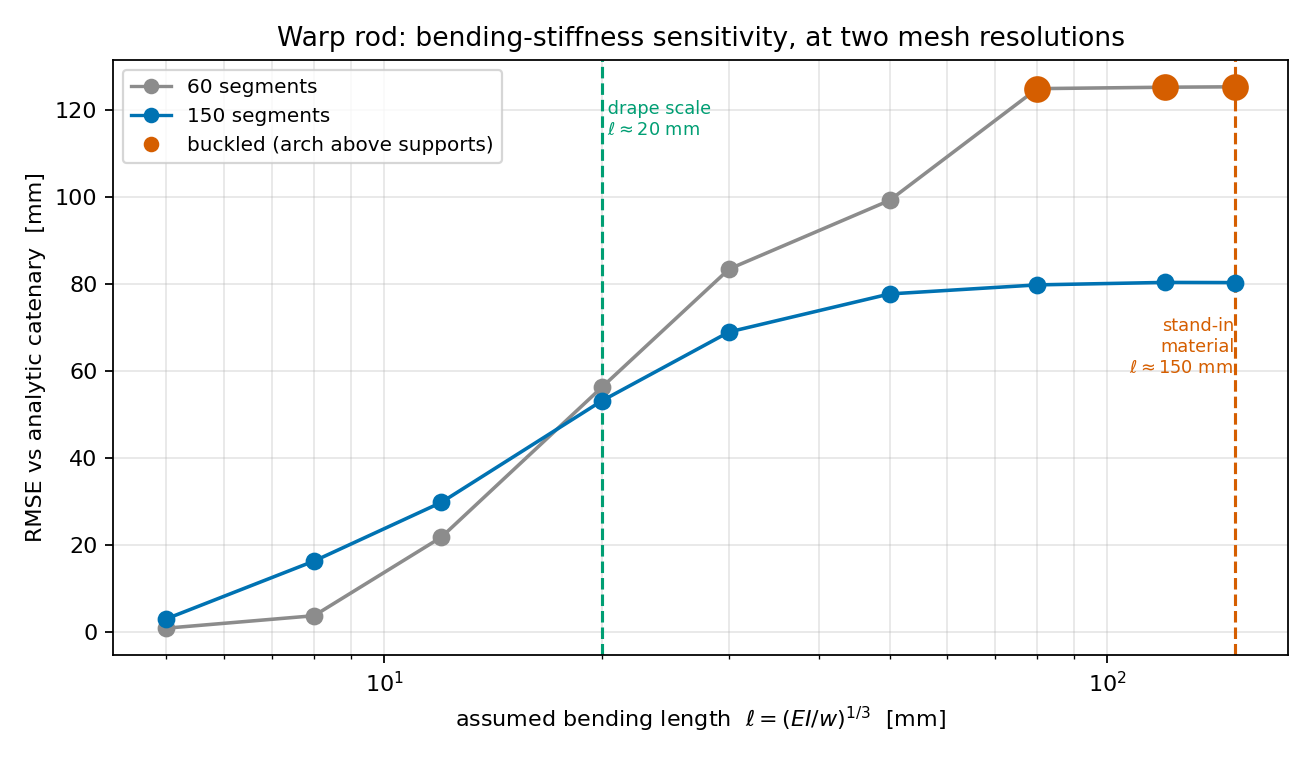
\includegraphics[width=0.78\linewidth]{warp_bend.png}
  \caption{Warp rod accuracy against the assumed bending stiffness, parametrised by the elasto-gravitational length $\ell=(EI/w)^{1/3}$, at two mesh resolutions. Both curves rise with stiffness: the stand-in material ($\ell\approx150$~mm) is worst, the cable's $\sim$2~cm rounding scale ($\ell\approx20$~mm, used here) is far better and is read from the rounding, not fitted to the catenary. Only the coarse mesh buckles into an arch above the supports at high stiffness (orange); refining it leaves a milder under-sag --- so the buckle was a discretisation artefact, the stiffness sensitivity is not.}
  \label{fig:warpbend}
\end{figure}


\section{Provenance of the inputs}

\begin{table}[htbp]
\centering\small
\begin{tabular}{lll}
\toprule
field & source & value \\
\midrule
    \texttt{cable.length\_m} & measured & 0.8932 \\
    \texttt{supports.mid\_fraction} & measured & 0.4688 \\
\bottomrule
\end{tabular}
\caption{Which inputs were measured from the photograph and which were
assumed. Recorded automatically for every run.}
\end{table}

\section{Validity}
\label{sec:validity}

\paragraph{Frame calibration.} The cable's two ends are located
geodesically --- breadth-first search across the mask itself, twice --- rather
than as its leftmost and rightmost pixels. The distinction matters here: the
tape clamps the cable's \emph{angle} as well as its position, so a slack
cable leaves the clamp along the tape's direction and bends back, carrying it
horizontally \emph{past} its own anchor (86\,px in this photograph). Taking
the horizontal extreme therefore picks a point on the descending cable rather
than the clamp.

An earlier version did exactly that at one end while the other came from where
tracing halted --- two ends defined by two different rules --- and the
resulting frame was tilted enough to place two physically level clamps 81\,mm
apart in height. With both ends found by one rule, and the clamp-to-clamp line
adopted as the horizontal (the clamps are level in the apparatus, so this also
removes camera roll, here $-0.40^\circ$), that difference is now $0.0$\,mm by
construction.

\paragraph{Independent check.} The frame is fixed by the two OUTER clamps
alone, so the middle clamp is free to disagree, and is therefore a genuine
test. It is recovered at $x = 0.164$\,m against $0.150$\,m measured by tape ---
$14$\,mm, or 4\% of the span --- and $3.9$\,mm above the outer clamps against
$0$ expected. Neither is forced by the calibration. The residual is consistent
with hand-measuring the clamp positions and with lens distortion toward the
frame edges, and it bounds the accuracy of any
simulation-versus-photograph comparison below.

\paragraph{Independent reproducibility.} The same physical cable was photographed a second time in a different rig --- 2 clamps spanning $0.350$\,m rather than 3, a different camera orientation, and an independent scale calibration ($193.109$ vs $164.161$ \textmu m per pixel). Passed through the identical extraction, its free length comes out $L = 0.8929$\,m against $L = 0.8932$\,m here: a difference of $0.32$\,mm on a $893$\,mm cable, $0.036\%$. Two independent measurements of one object agreeing to a third of a millimetre is the strongest available evidence that the length the simulations are scored against is real and not an artefact of one photograph. The central inversion reproduces as well. The Newton cable method, which is the most faithful to the mathematics, reaches $1.51$\,mm against the analytic curve in the cross-check and $0.91$\,mm here, yet sits $71$\,mm and $75$\,mm from the two photographs respectively. The solver that nails the ideal curve stays far from the real cable in \emph{both} geometries, so the gap is not an artefact of the middle clamp in the primary experiment --- it appears already in the simplest single-span rig.

\paragraph{What the model-free check says.} The traced arc length exceeds the
length implied by fitting catenaries to the measured sags by roughly 58\,mm.
This is not numerical: it is the clamped end again. A catenary meets its
support at whatever angle the length demands, while the tape forces a
different angle and the cable bends to accommodate it, and that bend costs arc
length the catenary does not spend. It is the largest single modelling
discrepancy in this study and is a property of the apparatus, not of any
solver.

\paragraph{Results that do not depend on the photograph.} The following rest
on the mathematics and the simulations alone, and are unaffected by any
measurement made from the image:
\begin{itemize}
  \item the verification of~\eqref{eq:catenary} against its closed form;
  \item every solver's error against the analytic catenary;
  \item the hyperparameter sweep and its conclusions;
  \item the Warp rod's stiffness sensitivity, and that its coarse-mesh buckle is
        a discretisation artefact the finer mesh removes (the \emph{choice} of
        the floppier, drape-consistent stiffness uses the photograph, but these
        do not).
\end{itemize}

\paragraph{Modelling limits.} The catenary is the $EI \to 0$ limit. The real
cable is a charger cable with a permanent set, so its rest shape is not
straight and some deviation from any ideal curve is physical rather than
numerical. The tape also clamps the cable's angle, which the classical
catenary does not model. Both effects are concentrated near the clamps, and
both are measurable, which makes them results to quantify rather than caveats
to apologise for.

\section{Conclusions}
\label{sec:conclusions}

The solver that best reproduces the mathematics is not the one that best matches the photograph: Newton cable - point pin (kink) attains 0.91~mm against the analytic curve but 75.1~mm against the real cable, while PhysX capsule chain (D6) is the reverse (74.4~mm and 32.8~mm). This is the central result, and it is a statement about BOUNDARY CONDITIONS rather than about solver quality --- see Section~\ref{sec:conclusions}.

\paragraph{Why the ranking inverts.} The photographed cable is held with
tape, which fixes the direction in which the cable leaves the clamp. The
classical catenary imposes no such condition: it meets its support at whatever
angle the length happens to demand. These are different boundary-value
problems on the same differential equation, and they have different solutions
near the clamps.

Three independent observations support this reading rather than "one solver is
simply better". First, the traced arc length exceeds the length implied by the
measured sags by roughly 58\,mm --- extra cable spent bending to satisfy an
imposed angle, which a catenary never spends. Second, the discrepancy is
concentrated near the clamps and not distributed along the span. Third, the
method that agrees most closely with the photograph is not the more accurate
solver by any other measure; it is simply the one whose own error happens to
lean the same way.

A solver that reproduces the analytic catenary to a millimetre is therefore
behaving correctly. The residual against the photograph is a property of the
apparatus, and closing it requires changing the MODEL --- imposing the clamped
end --- not the solver or its settings.

\paragraph{What this argues for methodologically.} With only simulation and
photograph, the natural conclusion would have been that the most accurate
solver was the least accurate, and effort would have gone into tuning a solver
that was already right. The analytic leg is what distinguishes numerical error
from modelling error, and it costs no experiment: it is available in closed
form for exactly the idealisation the solvers claim to implement. That is the
argument for carrying all three.

\paragraph{Sharpening the claim.} It is not that the simulations use pinned
ends and the apparatus uses clamped ones. Every method here \emph{welds} its
end bodies, so all of them impose a clamped end. The difference is the ANGLE at
which it is clamped: the simulations start from the analytic catenary and
therefore weld the ends at the catenary's own exit angle, whereas the tape
holds the real cable close to vertical. Same boundary condition type, different
boundary value --- and it is the value that the residual measures.

\paragraph{The test, carried out.} The middle support admits the check directly. A strip of tape does not pin the cable at a point; it holds a short segment flat against the door, so the cable leaves the support horizontally and its bending stiffness rounds the top --- whereas a point pin forces two catenary spans to meet with opposite slopes in an unavoidable upward kink (a catenary's only horizontal tangent is its lowest point, and the middle support is a high one). Figure~\ref{fig:overlay}, inset, shows the photograph rounding over exactly as the tape model does and the point pin cornering. Replacing the pin with the flat-tape condition moves the Newton cable from $75$~mm to $65$~mm against the photograph while moving it from $0.9$~mm to $21$~mm against the analytic catenary. That is the signature the account predicts: the more faithful boundary condition is FURTHER from the idealised curve and CLOSER to the real cable. The residual is a model choice, and correcting the model closes part of it --- without touching the solver or its settings.

\paragraph{The pinned-support check.} The obvious check --- rerun with a truly
pinned rather than clamped middle support --- cannot be done in Newton: its
\texttt{add\_rod} exposes capsule BODIES rather than nodes, and every way of
holding a body also holds its orientation, so \texttt{--mid-support pin}
returns a \emph{bit-identical} result (same sag to 0.1\,mm, same error to
0.01\,mm) and a true position-only pin cannot be expressed through that API at
all; the repository's own \texttt{clamp\_indices} documents this. The Warp rod
\emph{can} express it --- a node of zero inverse mass constrains position
alone --- and once it is given a bending stiffness in the cable's own floppy
regime (Figure~\ref{fig:warpbend}) it does exactly that: it pins the middle
position, leaves both tangents free, and its bending then rounds the support
just as the tape model and the photograph do (Figure~\ref{fig:overlay}, inset).
That rounding, reached from a genuine position-only pin rather than an imposed
flat clamp, is the independent confirmation Newton's API cannot provide.

\paragraph{Extending the test to the outer clamps.} The same idea applies at
the two end supports, where the pinned-versus-clamped API limitation above does
not obstruct it: impose the MEASURED end tangent rather than the catenary's. The
angle at which the cable leaves each outer clamp is directly readable from the
photograph, and welding the end bodies at that angle would move the simulation
further toward it. The residual would not close entirely --- the cable's
permanent set, a charger cable's memory of its coil, is a rest-shape effect no
boundary condition can represent, and it is the most likely floor on any
sim-to-photo agreement. Separating that floor from the remaining
boundary-condition error is the natural next step; the middle-support result
above shows the method works.

\end{document}
